% ======================================================================
\section{\lstinline{TODO}}

% ======================================================================
\subsection{Getting started}

% ----------------------------------------------------------------------
\begin{frame}[fragile]{A few demos}

  Directory \lstinline{doc/demo} contains examples of various types of genericity for {\em lists}.

  \begin{itemize}
  \item These are shorter, focused snippets;
  \item Use them as a basis for the part of your report explaining how genericity may be implemented in C, also with their preferred use cases.
    \begin{itemize}
    \item We give you code, you write your own course notes!
    \end{itemize}
  \item Feel free to {\em not} understand everything first time.
  \end{itemize}

  Learning to write {\em about} code is just as important as writing it.
  
\end{frame}


% ----------------------------------------------------------------------
\begin{frame}[fragile]{Resizable arrays (\texttt{src/ds/array.c})}

  \begin{enumerate}
  \item Study the interaction between \lstinline{include/ds/array.h}, \lstinline{src/ds/array.c}, and \lstinline{test/1-array.c}
    \begin{itemize}
    \item Make a diagram of the memory areas at play (header, slots), particularly during a resize operation;
    \item Pay attention to pointer tagging, observe how iterators are constructed;
    \item Understand where/why \lstinline{memset()}, \lstinline{memcpy()} and friends are useful; 
    \item The test summarizes most of the properties that other modules will need.
    \end{itemize}
  \item A few functions must be completed in \lstinline{src/ds/array.c}, check whether your proposal is OK with:

    \lstinline{make test/1-array@check}

  \item Write down a recap of the techniques used: type of genericity, hidden metadata.

  \item Once your arrays behave correctly, that unlocks the basic versions of a few maps.
  \end{enumerate}

  Bottom line: You should spend much more time reading code than writing it.
  \begin{itemize}
  \item Formulating your questions is an {\em excellent} exercise.
  \end{itemize}

\end{frame}


% ======================================================================
\subsection{Map options}

% ----------------------------------------------------------------------
\begin{frame}[fragile]{General map options}

  Make live memory scans (JTAG, shared/leaked mem.) more difficult for an opponent:

  \begin{itemize}
  \item \lstinline{ds_secure_removal}

    Whether to reset mapping memory after \lstinline{map_remove()}. Already implemented.

    {\em Note:} Popularized by GrapheneOS (and Molly!)
    
  \end{itemize}
  
  More often than not, the same key gets probed several times in a row.
  
  \begin{itemize}
  \item \lstinline{ds_mtf}

    If a data structure uses some form of chaining, a common trick is to swap the last key found with its chain (list) head. To be used primarily with \lstinline{ds_ht_chained} addressing (below.) Also useful with hashtries or coalesced designs like Verstable.
    
    {\em Note:} Also called {\em Ryabko's bookstack}, instrumental in the \lstinline{bzip2}/\lstinline{xz} compressors.
  \end{itemize}  

  All data structures involving a hash may use the following options:

  \begin{itemize}
  \item \lstinline{hash_no_finalize}: Disable the (Fibonacci) hash finalizer. Already implemented.
    
  \item \lstinline{hash_filtered}: Skip call to equality test if hashes mismatch.
    
  \end{itemize}

\end{frame}


% ----------------------------------------------------------------------
\begin{frame}[fragile]{General recursive structure options}

  Recall that \lstinline{ds_backend_nodes} is defined to be $\log_2$ of the arity.
  
  \begin{itemize}
  \item \lstinline{ds_nd_list}: Already implemented, with sorted variant.

  \item \lstinline{ds_nd_bst}: Binary search trees.

    All tree structures need deep understanding of the map code: working with addresses inside slots, with their store subject to resizing (and therefore address change), is challenging yet of course doable.
    
  \item \lstinline{ds_nd_treap}

    Actually an option of the above: whether to use the hash for randomized balancing. Much of the BST code could be factored out.

  \item \lstinline{ds_nd_hashtrie}: Use plain hash bits as n-ary tree routing info.

    If all hash bits are consumed, natively degenerates into list collision chaining.

    {\em Note:} Yet \href{https://nullprogram.com/blog/2023/09/30/}{another elegant idea by Chris Wellons}! Also check \href{https://en.wikipedia.org/wiki/Hash_array_mapped_trie}{HAMT} structures.
  \end{itemize}

\end{frame}


% ----------------------------------------------------------------------
\begin{frame}[fragile]{General hashtable options}

  All hashtables already honor the following options:
  \begin{itemize}

  \item \lstinline{ds_ht_primes}

    Whether to use primes equal 3 (mod 4) instead of powers-of-two for \lstinline{dim}.

    See \lstinline{test/1-map.c} if you want to generate other primes.
    
  \item \lstinline{ds_ht_modulo_fast}: If \lstinline{dim} is a power-of-two, replace {\em modulo} with {\em and}.

    {\em Note:} Make sure to check the works of Daniel Lemire!

  \item \lstinline{ds_ht_lf_min}, \lstinline{ds_ht_lf_max}

    Bounds for the {\em load factor}, the ratio of \#tombstones plus \#mappings over \lstinline{dim}.

    Used to trigger resizes on \lstinline{map_put()} and \lstinline{map_remove()}.

    Different backends will accomodate different ranges for the upper bound.

  \item \lstinline{ds_ht_chained}, \lstinline{ds_ht_quadratic}, \lstinline{ds_ht_linear}, \lstinline{ds_ht_robin_hood}

    Actual hashtable addressing backend (options are mutually exclusive.)

    {\em Robin-Hood} has been set aside {\em linear} in order not to clutter the latter.

  \end{itemize}

\end{frame}


% ----------------------------------------------------------------------
\begin{frame}[fragile]{Open-addressing hashtable options}

  Open addressing may use tombstones (that's the default, easy way to go.)

  \begin{itemize}

  \item \lstinline{ds_ht_tomb_reuse}: Whether tombstones are reused.

    Virtually all open addressing variants may choose to reuse tombstones.

  \item \lstinline{ds_ht_tomb_none}

    In the specific case of linear probing (including Robin-Hood), it is even possible to avoid tombstones completely. But it's {\em not} trivial!

    {\em Note:} Knuth's Algorithm R for standard linear probing may not be the one to use for Robin-Hood! The Java implementation is a good starting point.
  \end{itemize}

  Linear probing (but not Robin-Hood!) may try to reduce primary clustering by {\em salting} (randomizing) the displacement for the next probed index.
  
  \begin{itemize}

  \item \lstinline{ds_ht_hash_salted}

    Add a few bits of the key hash in the probe displacement.

    If all hash bits have been consumed, defaults to 1 (standard linear probing.)

    {\em Note:} Trick was used until early Python 3.x series for the core dictionary structure.
  \end{itemize}

\end{frame}


% ======================================================================
\subsection{Moving forward}

% ----------------------------------------------------------------------
\begin{frame}[fragile]{\lstinline{apman$ ./maplab --experiment textbook --preset tiny}}

  But first, compile benchmark execs: \lstinline{apman$ make}
  
\begin{center}
  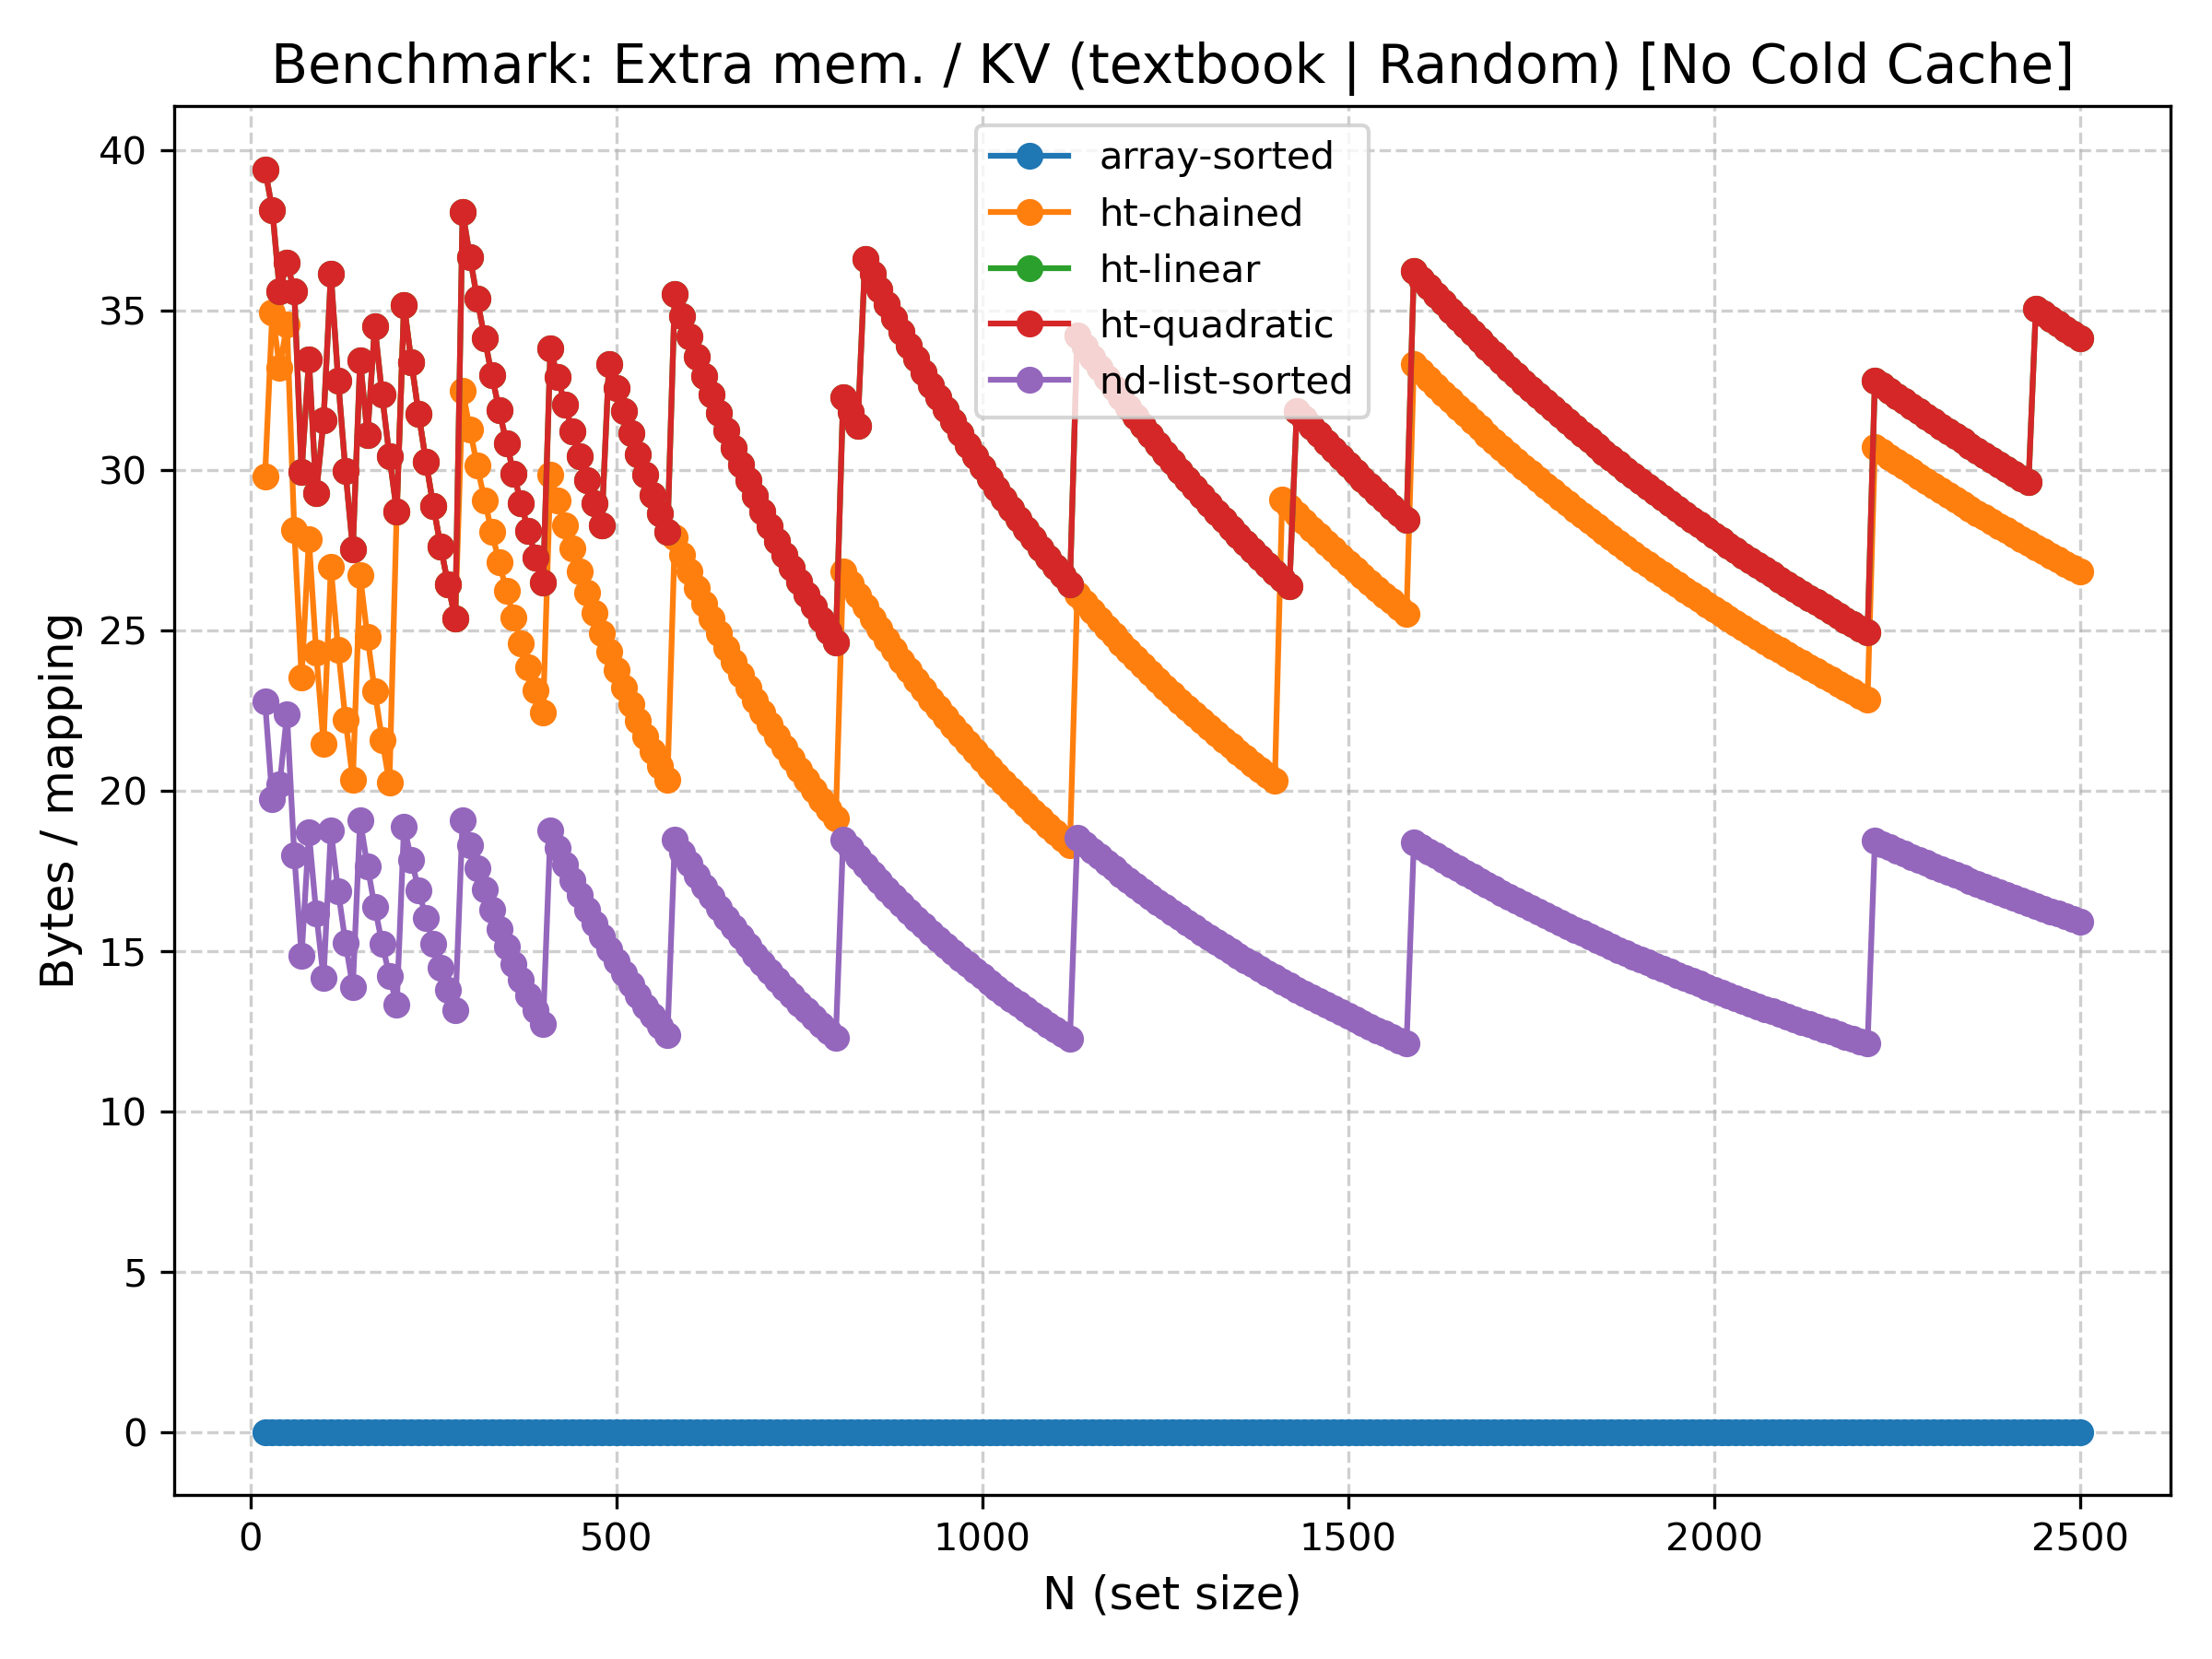
\includegraphics[scale=.3]{fig/plot_mem_nocold_abpkv.png}
  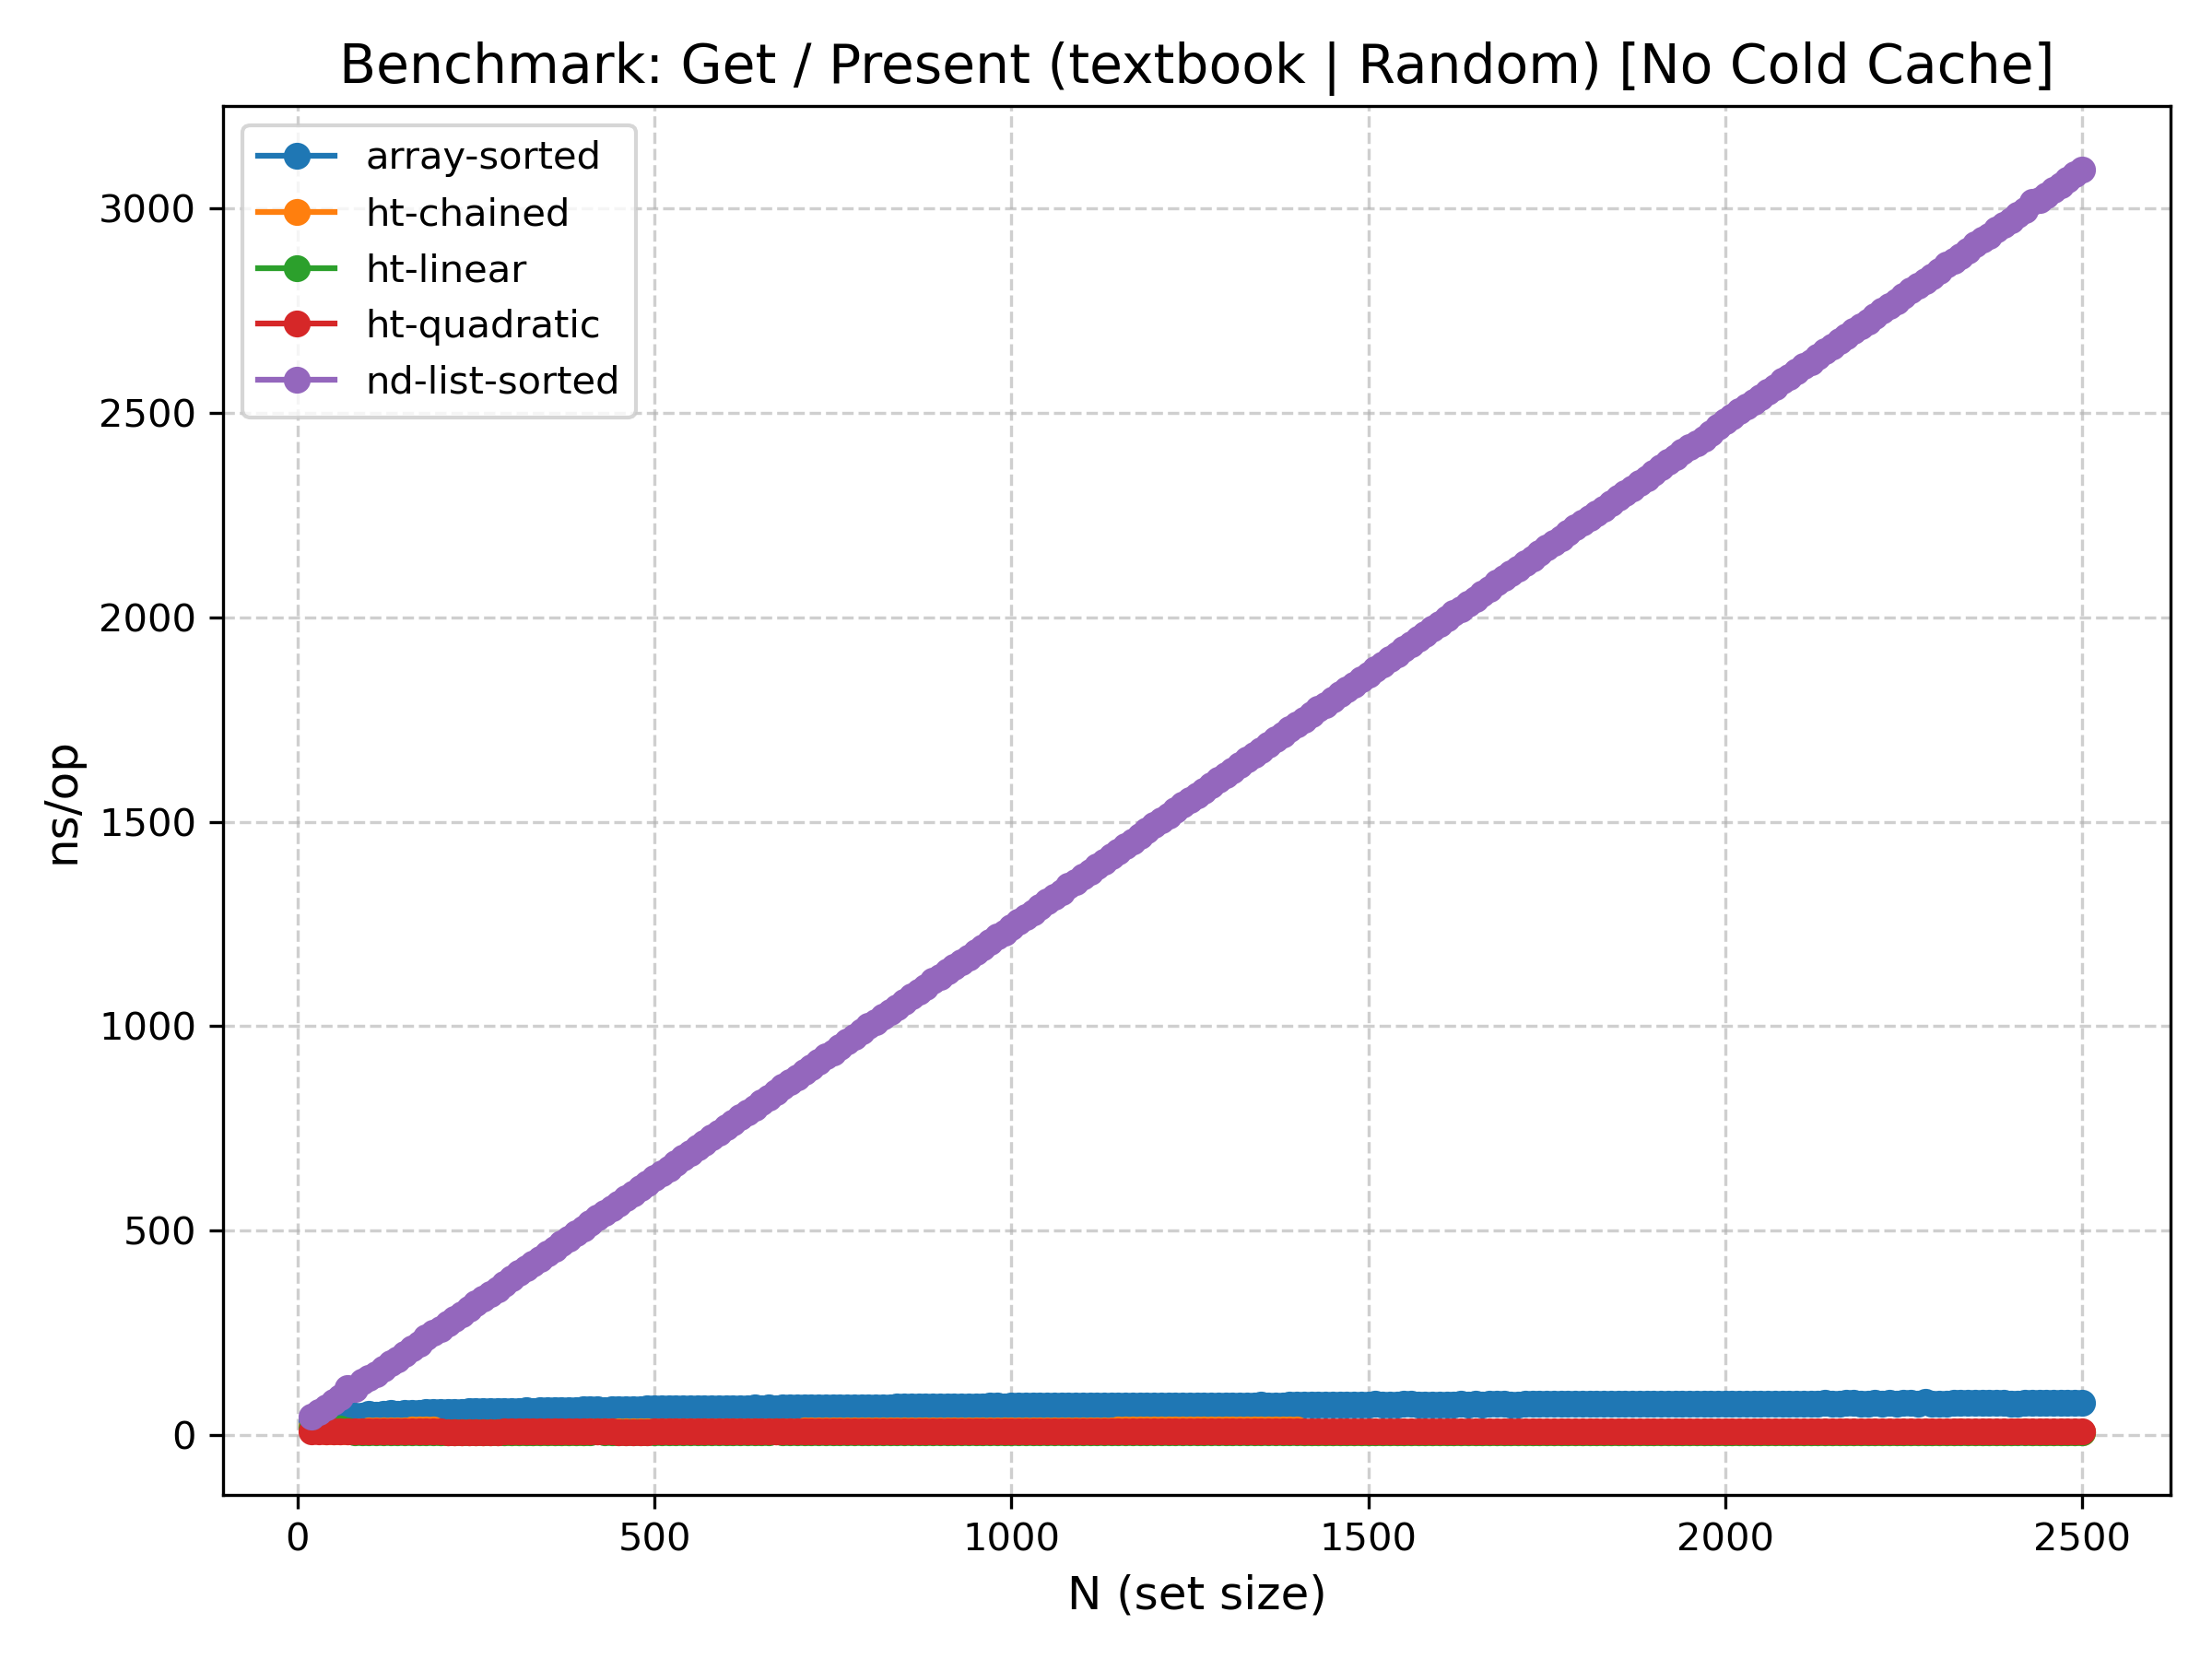
\includegraphics[scale=.3]{fig/plot_time_nocold_get_present.png}
\end{center}

\begin{itemize}
\item Once you've explained these plots and you're convinced linear-time is unusable:
  \begin{enumerate}
  \item Remove directory \lstinline{experiment/textbook/output} (or rename it to keep it.)

  \item Remove \lstinline{textbook-nd-list-sorted} from \lstinline{experiment/textbook/benchmark}
  \item Use more data: \lstinline{apman$ ./maplab --experiment textbook --preset small}
    
  \end{enumerate}
\end{itemize}

\end{frame}


% ----------------------------------------------------------------------
\begin{frame}[fragile]{\lstinline{apman$ ./maplab --experiment textbook --preset tiny} (cont'd)}

  For the radar plot: outer is better, solid line is median, shaded area is IQR.
  
\begin{center}
  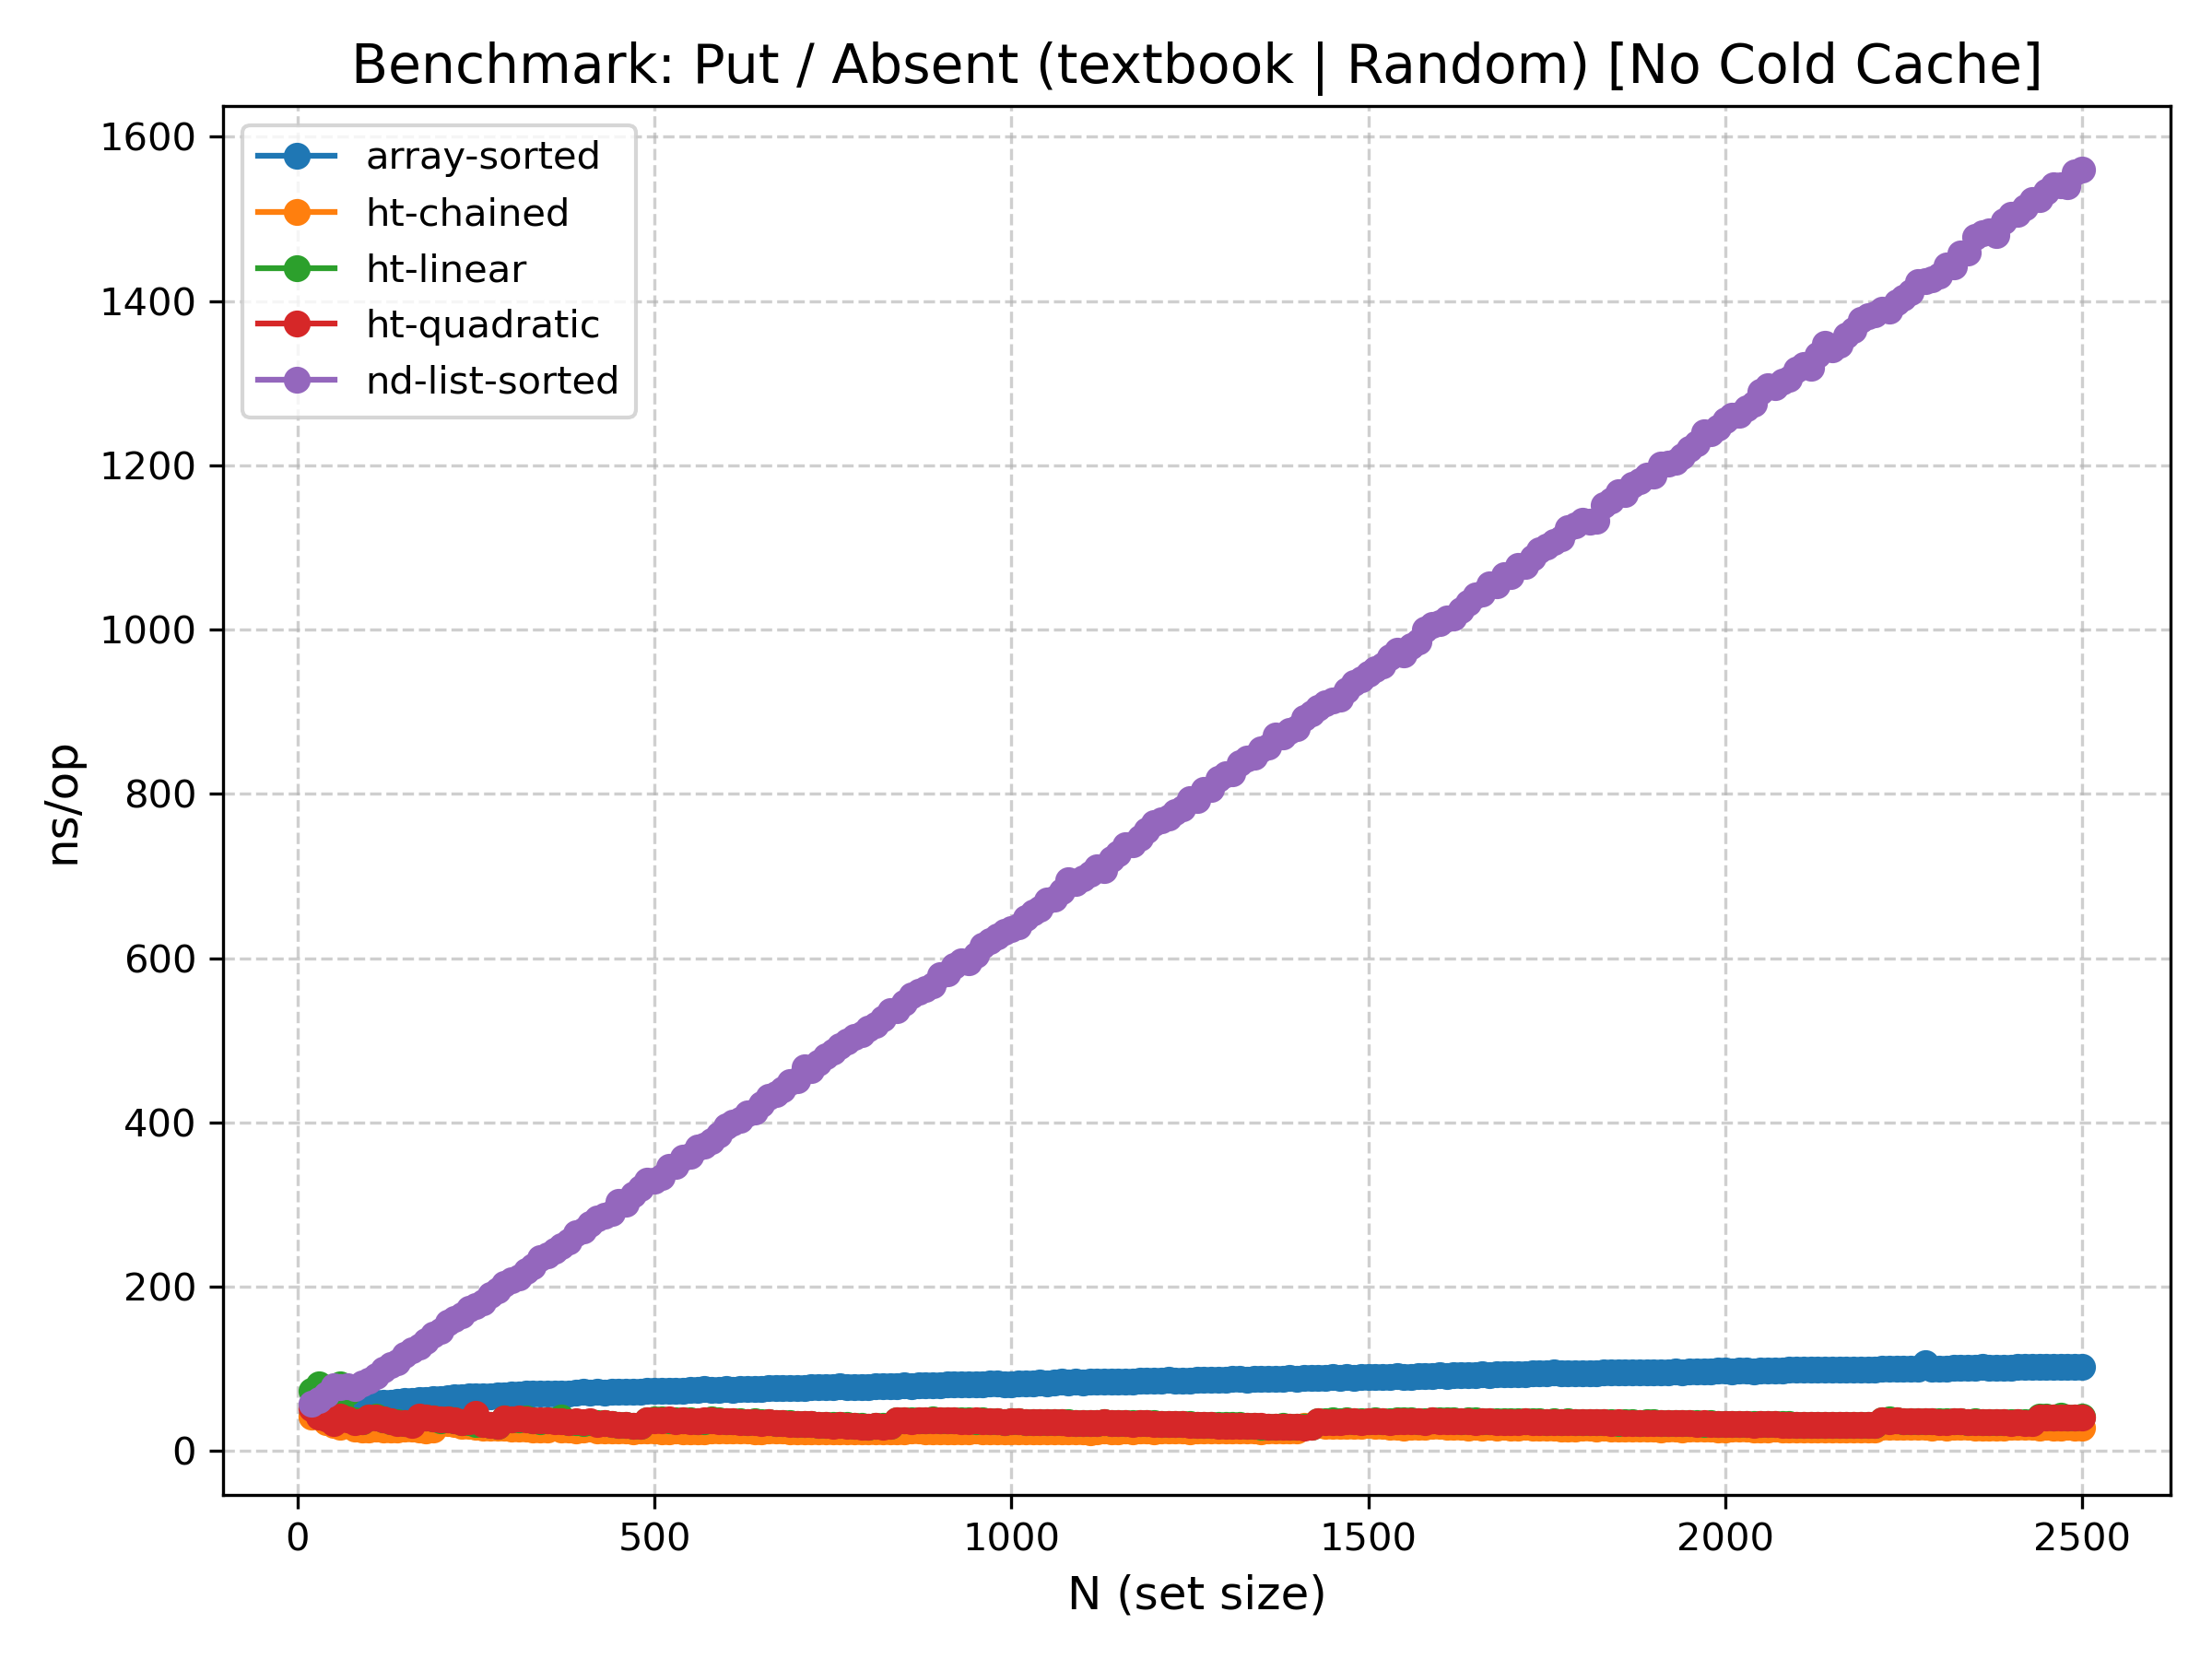
\includegraphics[scale=.3]{fig/plot_time_nocold_put_absent.png}
  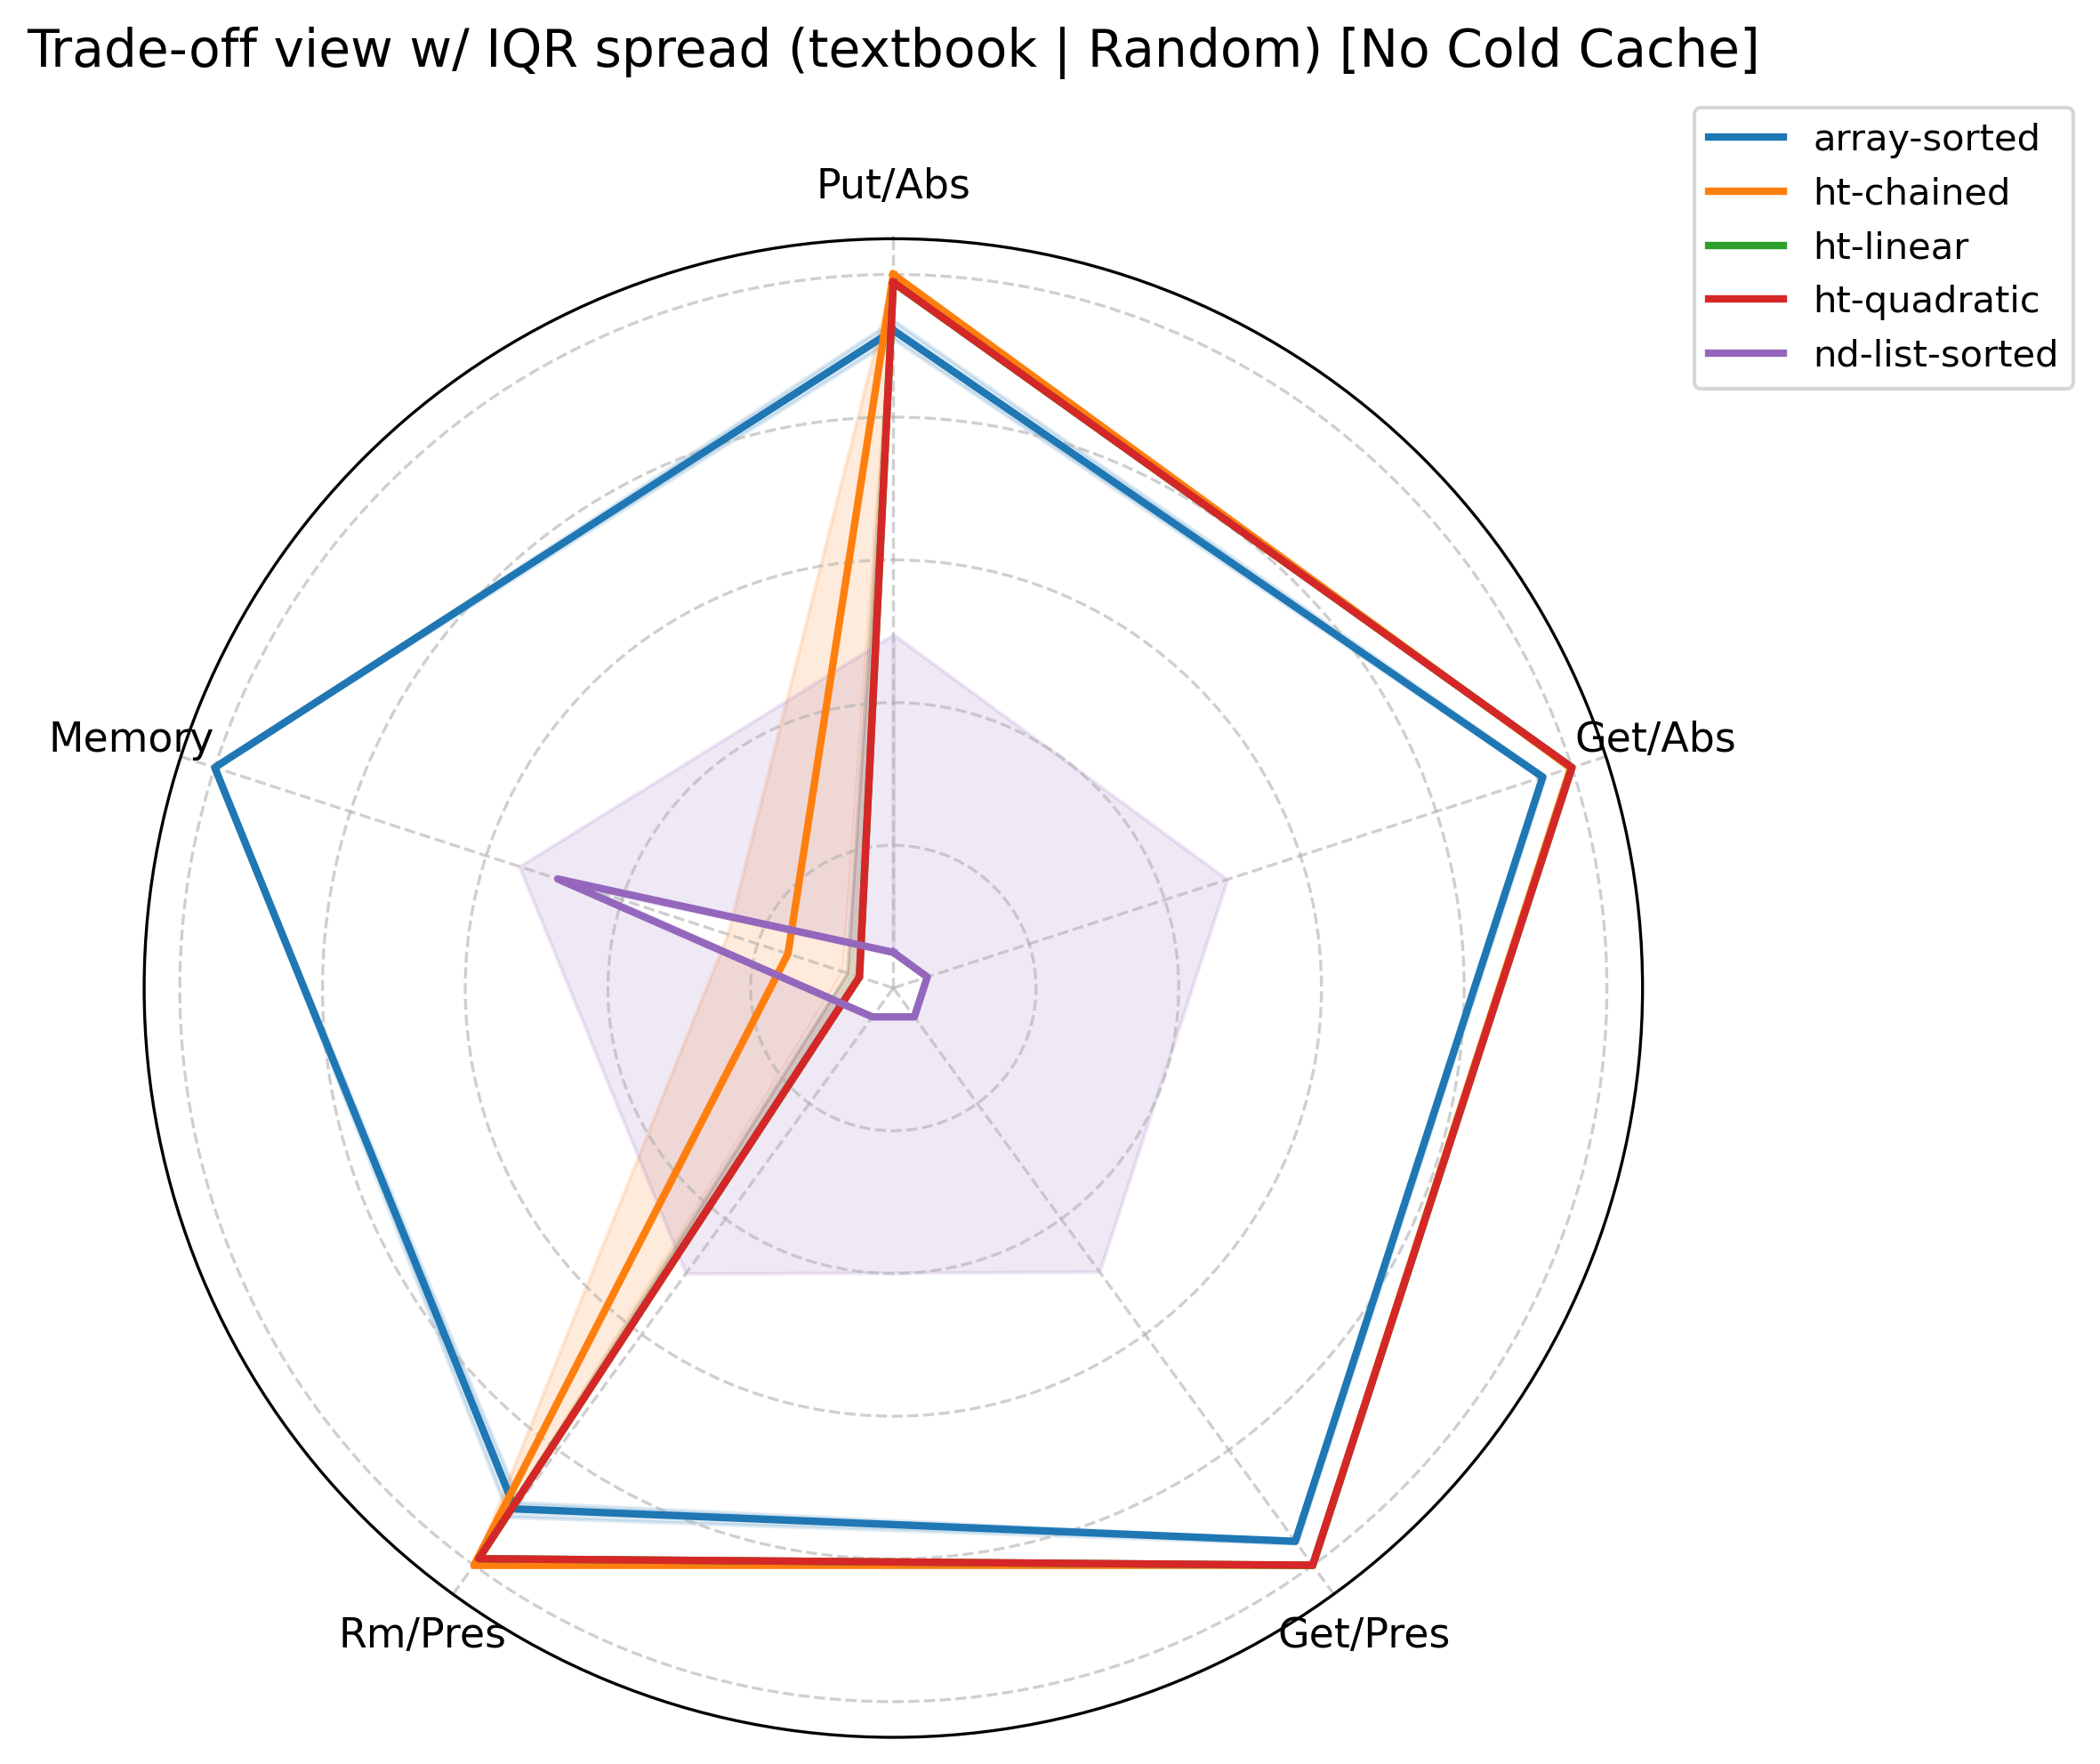
\includegraphics[scale=.3]{fig/radar_nocold_tradeoff.png}
\end{center}

\begin{itemize}
\item With options \lstinline{ds_secure_removal}, \lstinline{ds_ht_primes}, \lstinline{hash_no_finalize}, \lstinline{ds_ht_modulo_fast}, \texttt{ds\_ht\_lf\_\{min,max\}} already implemented, you can exercise benchmarking to draw a number of conclusions {\em today}.
\end{itemize}

\end{frame}


% ----------------------------------------------------------------------
\begin{frame}[fragile]{Maps}

  Learn how to {\em use} the environment and the methodology first.

  All while concentrating on implementing your best maps. In higher-level C.

  That should account for up to 70\% of the project.
  
  \begin{enumerate}
  \item Implement, test and benchmark map variants in:

    \texttt{include/ds/map/backend/\{chained,linear,quadratic,bst,hashtrie\}.h}
    
    This part of your report will basically be a plain textbook on algorithms.

    Your report should ask and answer the right questions with empirical evidence.

    See the \lstinline{README.md} for how to design and run map experiments.
    
  \item Download some real serious external code

    {\em Integrate} it in the benchmarks, {\em as seamlessly as possible}. Explain how you did.
    
    Give the wonderful {\em Verstable} map a try!

    Quadratic addressing with coalesced chains and {\em relative} pointers\dots

    Exercise your skills in C templating. You're only a couple \lstinline{#define}'s away!

  \end{enumerate}

  Those two steps ensure you master the coding standards at a reasonable level.
  
\end{frame}


% ----------------------------------------------------------------------
\begin{frame}[fragile]{Maps (cont'd)}

  You may also want to reflect on the methodology itself:
  
  \begin{enumerate}
  \item Feel free to dissect, criticize, evolve the tests or the benchmark

    Explain why and how you did (also to validate your approach.)

    For example, the benchmark cannot measure the effect of Move-to-Front.

    Also, the unit tests could be slightly more stringent. 

  \item Same for the map code

    You may want to handle insertion order more thoroughly (tombstones.)

    Also, it lacks proper de/allocation for the \lstinline{control} bytes!

  \end{enumerate}

\end{frame}


% ----------------------------------------------------------------------
\begin{frame}[fragile]{Add more (simpler!) data structures}

  \begin{enumerate}
  \item Add the {\em deque} data structure:
    \begin{itemize}
    \item Backends: resizable arrays {\em vs.} intrusive links (see)
    \item Upstream abstract data types: lists, stacks, queues
    \item Design the interface, the implementations, the tests and the benchmarks
    \item Explain the typical use cases.
    \end{itemize}

  \item {\em Embedded specials}
    \begin{itemize}
    \item Add a bip-buffer! Explain why it may be useful.
    \item Consider the resemblance with a general arena allocator\dots
    \item Map-related: implement Cuckoo hashing
    \end{itemize}
    
  \end{enumerate}

  Once you've followed the OS course, think of adding:
  \begin{itemize}
  \item A thread pool;
  \item Asynchronous computations with \lstinline{future_t}'s
  \item You may then start diving into the harsh world of {\em concurrent} data structures\dots
  \end{itemize}
  
\end{frame}


% ----------------------------------------------------------------------
\begin{frame}[fragile]{Typical report outline}

  A report skeleton is given in \lstinline{doc/report}.
  \begin{itemize}
  \item Pay attention to the many references you may want to explore!
  \end{itemize}

  We expect a discussion of the following points, backed by benchmarks where relevant:
  \begin{enumerate}
  \item Genericity: why and how?
  \item Arrays: why and how?
  \item Maps on unsorted data
    \begin{itemize}
    \item Hashtables
    \item Hashtries
    \end{itemize}
  \item Maps on sorted data
    \begin{itemize}
    \item Search trees
    \item Binary search
    \end{itemize}
  \item Deques
    \begin{itemize}
    \item Design of the data structure, of the tests, and of the benchmark
    \item Discussion of the sentinel technique for the link-based backend
    \end{itemize}
  \end{enumerate}

\end{frame}


% ----------------------------------------------------------------------
\begin{frame}[fragile]{What {\em we} will pay attention to}

  For example: 
  \begin{itemize}
  \item Could your report be used as a reference for other students?
  \item Quality, coverage, and validation/refutation of your hypotheses (maps)
  \item How the techniques we introduced were adapted (deques)
  \end{itemize}

  We show you a (vast) landscape, show us how you explore it scientifically!
  
\end{frame}


